\documentclass[a4,12pt]{scrartcl}

\usepackage{xltxtra,color,tabularx,graphicx}

\usepackage[english]{babel}

\usepackage{hyperref}
\hypersetup{colorlinks=true, citecolor=red, linkcolor=blue, urlcolor=green, breaklinks=true}

\usepackage{natbib}
\bibpunct[: ]{(}{)}{;}{a}{}{;}

\usepackage{gb4e}


%%%%%%%%%%%%%%%% TEST + küsse %%%%%%%%%%%%%%%%%

%%%%%%%%%%%%%%%%%%%%%%%%%%%%%%%%%%%%%%%%%%%
%
%				                              GUIDELINES
%
%%%%%%%%%%%%%%%%%%%%%%%%%%%%%%%%%%%%%%%%%%%
%
%GUIDELINES for the contributions to the volume “Semantic functions of complementizers in European languages”
%
%	COMPLEMENTIZER: “a word, particle, clitic or affix, one of whose functions it is to identify [a clause] as a complement” (Noonan 2007: 55).
%	COMPLEMENT MARKER: other kinds of expressions – e.g. whole constructions, word orders, prosodical featurs, etc. – which identify clauses as complements.
%	CANONICAL COMPLEMENTIZER (optional term): expressions that conform to Noonan’s definition (see above) AND occur only in finite complements.
%	Complementation Marker (identify finite+non-finite clauses as complements) > Complementizer (word/particle/clitic/affix which identify finite+non-finite clauses as complements) > Canonical Complementizer (Complementizer in *finite* clauses)
%
%General requirements
%Focus
%-	If your languages have equivalents of English that and if in Bob doesn’t know that/if Janet loves him, focus at least on these.
%-	If your languages DO NOT have equivalents of English that and if, focus at least on other finite-clause complementizers or complementation markers that are NOT identical to question words (e.g. English how, what).
%-	If your languages DO NOT have finite-clause complementizers or complementation markers, focus at least on complementizers or complementation markers which 1) are found in complements of propositional attitude predicates (‘think’, ‘believe’), knowledge predicates (‘know’, ‘learn’), perception predicates (‘see’, ‘hear’), and/or utterance predicates (‘say’, ‘tell’), and 2) are NOT identical to question words (e.g. English how, what).
%
%	Note:	You are free to discuss also question-word like complementizers, but the focus of the paper must include complementizers or complementation markers that are not like question words (provided, of course, such complementizers or complementation markers exist).
%
%Number of languages covered
%Contributions should preferably cover more than one language from the language family studied. This does not concern Basque, Maltese, Hungarian, Albanian, Greek, Romani and Kalmyk.
%%%%%%%%%%%%%%%%%%%%%%%%%%%%%%%%%%%%%%%%%%%%
\usepackage{authblk}

\title{Semantic and syntactic structure of complementizers in Saami languages}
\author[1]{Kristina Kotcheva}
\author[2]{Michael Rießler}
\affil[1]{Department of Linguistics, University of Konstanz}
\affil[2]{Scandinavian Department, University of Freiburg}

\begin{document}
 %%Contributions should be between 12,500 and 17,500 words long, including references.%KK: ca. 10–15 Seiten%

\tableofcontents

\newpage
\maketitle

\begin{abstract}
The chapter describes the the syntactic structure and semantic functions of complementizer constructions in three endangered Saamic (Uralic) languages.\\


{\bf Keywords:} semantics, syntax, typology, subordination, complementizer\\

{\bf ISO 639-3:} sjd, sme, sms 
\end{abstract}

\section{Introduction}
\subsection{Aim of the investigation}
\paragraph{Prospect I}  Our paper aims at a detailed description of the syntactic structure and semantic functions of complementizer constructions in North Saami, illustrated with minimal pairs (in concordance with the project description). North Saami data will be taken from existing descriptions \citetext{e.g. \citealt{nickel1994, sammallahti1998b, nielsen1979-1}} and corpora (\url{http://giellatekno.uit.no/text.en.html}).  %Are there restrictions on the co-occurrence of complementizers and e.g. modal markers?\\

\paragraph{Prospect II} We will also try to compare North Saami with Kildin Saami (E-Saamic<Uralic), for which syntactic and semantic descriptions are virtually non-existent. Kildin Saami data will be taken from a spoken language corpus (Kola Saami Documentation Project, DoBeS Archive. Nijmegen: Max Planck 
Institut for Psycholinguistics, \url{http://www.mpi.nl/DOBES/}) and from elicitations and experiments with native speakers.

\begin{itemize}
\item Section ?? Introduction
\item Section \ref{syntax} is rather descriptive and described the syntactic environments of complementizers - i.e. their FORM
\item Section \ref{semantics} is the main part of the present chapter, based on the syntactic description it describes the FUNCTION(S)
\item Section \ref{history} presents a rather short historical-comparative description, based on the previous section on the three Saamic languages
\item Section ?? summarizes the findings
\end{itemize}


\subsection{Saamic languages}

1.	briefly introduce the languages covered (among other things, mention possible characteristics of the languages as well as their genetic and geographical affiliation and – if possible – the number of speakers of the languages).

\begin{center}
\setlength\fboxsep{0pt}%sets padding thickness
\setlength\fboxrule{0.5pt}%sets border width
%\fbox{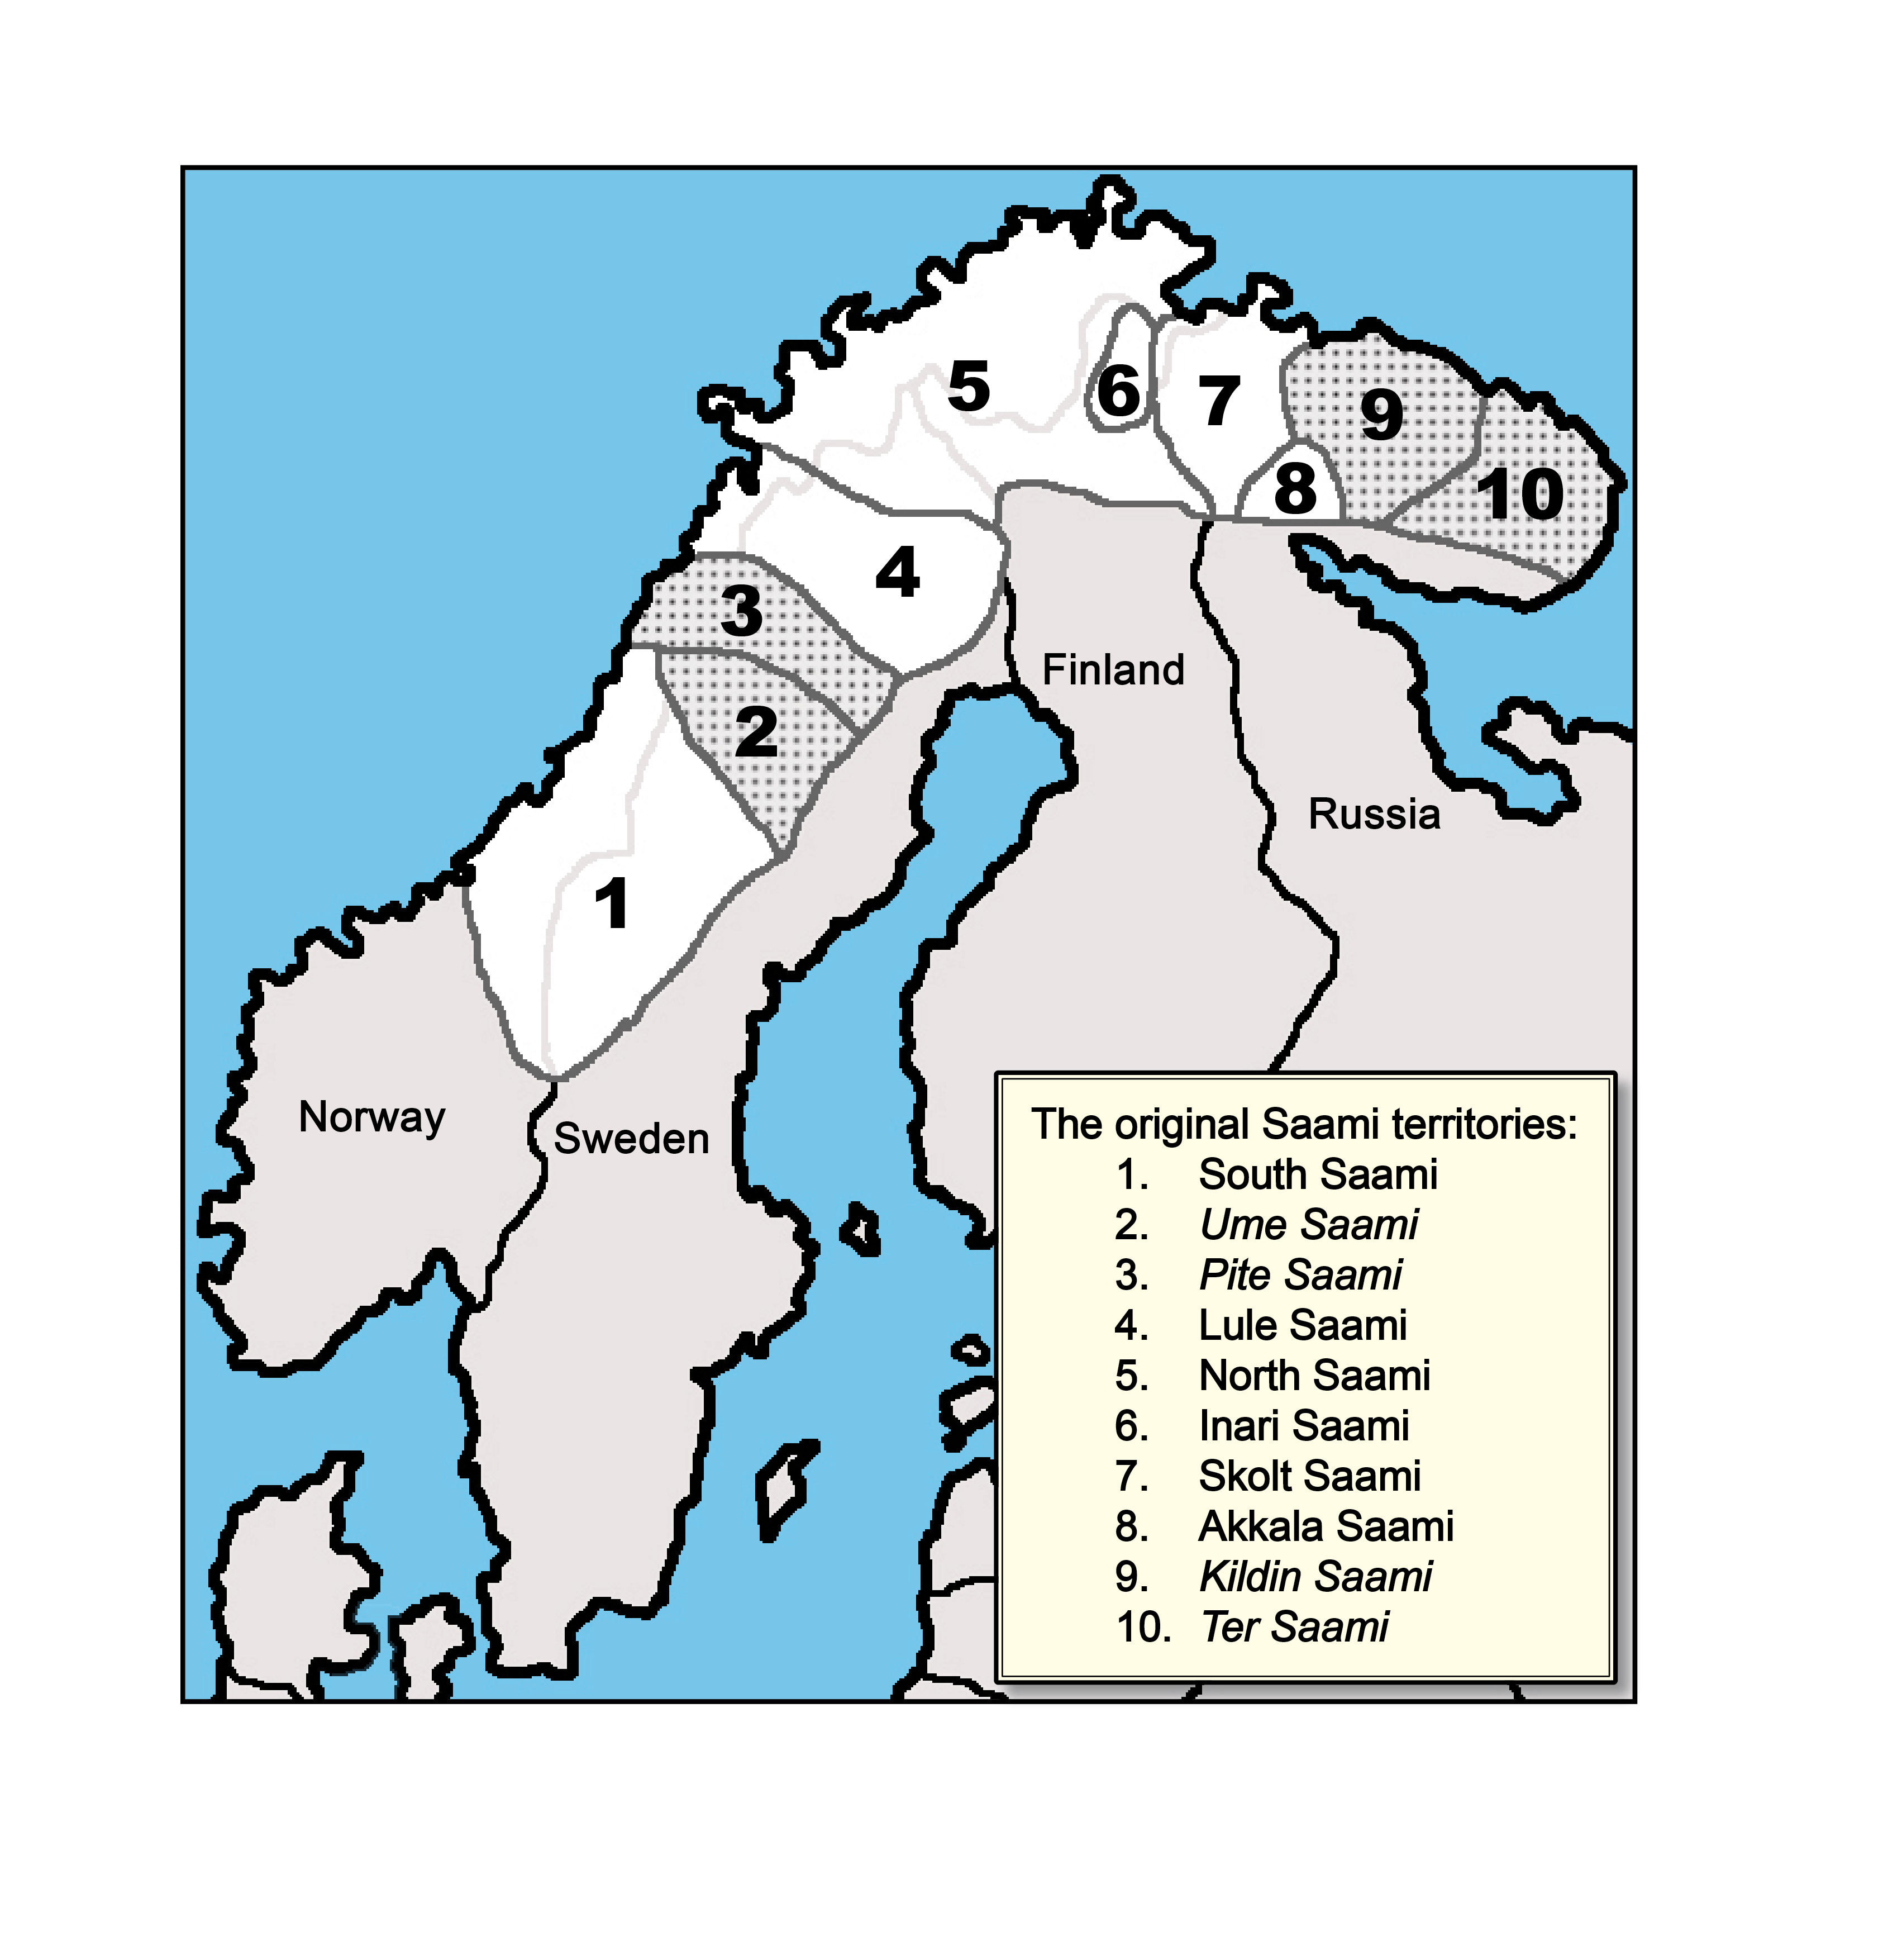
\includegraphics[width=60ex,height=38ex]{SaamiLgs.jpg}}
\end{center}

\subsection{Data used for this investigation}
North Saami
\begin{itemize}
\item Grammatical descriptions
\item Written corpora (GT)
\end{itemize}

Skolt Saami
\begin{itemize}
\item Grammatical descriptions
	\subitem Feist
	\subitem School grammar
\item Written corpora (Textsammlung mit CD)
\end{itemize}

Kildin Saami
\begin{itemize}
\item Grammatical descriptions
	\subitem Kert?
\item Spoken corpora (KSDP)
\end{itemize}

\section{Syntax of complementizers in three Saamic languages}\label{syntax}
%2.	give an overview of complementizers and complementation markers, including also e.g. equivalents of English how, what, etc.
KK: Tabellen am besten zusammenfügen

\subsection{North Saami}
\begin{table}[!ht]
\begin{tabular}{l | l l}
\hline
\hline
Nsaa & Gloss & Translation\\
\hline
{\bf ahte} & {\sc COMP} & 'that'\\
{\bf jos/jus} & {\sc COMP} & 'if'\\
{\bf go} & {\sc advCOMP} & 'when/if/because'\\
{\bf go} & {\sc attrCOMP} & 'that/which/than'\\
sahte & & 'if only'\\
vaikko/vaikke & & 'even if, even though'\\
\hline
\hline
\end{tabular}
\label{KompNSaami}
\caption{Complementizers in North Saami}
\end{table}

NSaa. {\it ahte} < Fin. {\it että} 'that' < FS pronominal stem {\it *e}- + modal suffix {\it -kta/ktä} 'so that'
 
NSaa. {\it go} < PSaa {\it *ko-} < FA {\it *ku-} 'as; than'

NSaa. {\it jos/jus} < Fin. {\it jos} 'if'

$\rightarrow$ {\it ahte} and {\it jos/jus} are Finnish loanwords in NSaa while {\it go} is inherited from pre-Protosaami \cite[226;245;251]{sammallahti1998b}.

In our paper we shall concentrate on {\it ahte}, {\it jos} and {\it go}. {\it Ahte} and  {\it jos}  function basically like English {\it that} (neutral) and {\it if} (uncertainty). {\it Ahte} can be combined with other subordinators (which shows that its meaning is neutral).  
{\it Go} is a polyfunctional adverbial subordinator (or “adverbalizer”) introducing temporal (\ref{goTemporal}) or causal (\ref{goCausal}) adverbial clauses.


\subsection{Kildin Saami}


\begin{table}[!ht]
\begin{tabular}{l | l l l l}
\hline
\hline
KSa 		& Gloss			&					&NSa translation	& English translation\\
\hline
šte		&{\sc COMP} ?		&< Russian {\it što}		&ahte			&'that'\\
%bydte	&				&					&ahte\\
jesli		&{\sc	 COMP} ?		&< Russian {\it jesli}		&jos				&'if'\\
%poke	&				&< Russian {\it poka}		&go\\
gū		&{\sc advCOMP} ??	&$\leftarrow$Proto Saamic&go				& 'XXX'\\
\hline
\hline
\end{tabular}
\label{KildinComps}
\caption{Complementizers in Kildin Saami}
\end{table}


\subsection{Skolt Saami}
%3.	mention which complementizers and/or complementation markers will be in focus in the remainder of the paper.
%4.	if relevant, consider the caveat that what is intuitively a complementizer need not be what actually identifies the complement as a complement.


\section{Semantics of complementizers in three Saamic languages}\label{semantics}% AT LEAST HALF OF THE PAPER
%1.	What are the semantic functions of – and contrasts between – the complementizers or complementation markers in focus (in addition to the function of embedding propositions/states of affairs in other propositions/states of affairs)? 
%		Note a:		Consider e.g. the following possibilities, some of which are discussed in the workshop description: i) contrasts between proposition (truth-valued) and state-of-affairs (non-truth-valued), ii) contrasts related to information structure, iii) contrasts related to knowledge, modality and adjacent phenomena (volitionality, implicativity, polarity), iv) temporal contrasts, v) aspectual (and Aktionsart) contrasts, vi) voice/valency-related contrasts.
%		Note b:	   Not only binary semantic contrasts may be found (for instance, between certainty and uncertainty), but also more complex semantic contrasts.
%		Note c:	   Complementizers or complementation markers may be semantically complex. For instance, we might find a complementizer or a complementation marker with both modal and aspectual meanings.
%2.	Are there minimal pairs which support the analysis of the semantic contrast? If yes, please exemplify, and please include examples with propositional attitude predicates, knowledge predicates, perception predicates, and utterance predicates, if relevant.
%3.	Are there other facts (co-occurrence restrictions, harmonic combinations, etc.) which support the analysis of the semantic contrast?
%
\subsection{Distribution}
\paragraph{Types of complements}%1.	In which types of complements are the complementizers or complementation markers in focus found?
\begin{exe}
	\ex Subject argument \label{ahteSubject} \citep[194]{nickel1994} 
	\gll 	Imaš 	lei, 	{\bf ahte} 	rámbuvrriin 	oaččui 	viine 	oastit.\\
	odd 	be:{\sc 3sg.pst} {\sc comp} shop:{\sc loc:pl} get:{\sc 3sg:pst} wine:{\sc acc:sg} buy:{\sc inf}\\
	\glt 	‘It was odd that one could buy wine in the shops.’
	
	\ex Object argument \label{ahteObject} \citep[194]{nickel1994}
	\gll 	Mun 	oainnán, 	{\bf ahte} 	áddjá 	lea 	boahtán.\\
	{\sc 1sg} see:{\sc 1sg} {\sc comp} grand\_father be:{\sc 3sg.prs} come:{\sc pastpart}\\%past participle
	\glt 	‘I see that grandfather has come.’
	
		 \ex Object complement \textbf{jos} \label{josObjekt}
	 	\begin{xlist}
		\ex 	
		\gll Mon in dieđe {\bf jos} mon gearggan boahtit.\\
		{\sc 1sg} {\sc neg:1sg} know:{\sc conneg} {\sc comp} {\sc 1sg} get\_ready:{\sc 1sg} come:{\sc inf}\\
		\glt ‘I don't know if I will manage to come.’ %’Jag vet inte om jag hinner komma.’ 
		
		\ex 
		\gll 	Mun 	oainnán, 	{\bf jos}  son áigu njuovvat sávzza.\\
		{\sc 1sg} see:{\sc 1sg} {\sc comp} {\sc 3sg} will:{\sc ind.prs} butcher:{\sc inf} sheep:{\sc acc.sg}\\
		\glt 	‘I shall see if s/he will butcher a sheep.’
		\end{xlist}	


	 \ex Relative clause \label{ahteRelativsatz} \citep[194]{nickel1994}
	\gll Sus lei jou geasset leamaš dat jurdda, ahte dáidá mus oažžut veahki.\\
	{\sc 3sg.loc} be:{\sc 3sg.ind.pst} already in\_summer be:{\sc pastpart} DEM:{\sc 3sg.nom} thought:{\sc nom.sg} REL may\_be{\sc 3sg.ind.prs} {\sc 1sg.loc} get:{\sc inf} help:{\sc acc.sg}\\
	'S/he had already in summer the idea that I might help him/her.'

	\ex \cite[195]{nickel1994}
	\gll De dáhpáhuvai, {\bf ahte} rievvár bođii.\\
	so happen:{\sc 3sg.ind.pst} {\sc advCOMP} robber:{\sc nom.sg} come:{\sc 3sg.ind.pst}\\
	\glt 'It happened that a robber came.'
	
	\ex Causal adverbial clause \label{goCausal}
%reviewer's note:  If one looks at the translation, the "final" clause introduced by /go/ seems rather a "causal" clause. *fertig*
\gll 	In 	sáhte 	boahtit 	{\bf go} 	lean 	buohcci.\\
	{\sc neg:1sg} can:{\sc conneg} come:{\sc inf} {\sc advCOMP} be:{\sc 1sg.prs} sick:{\sc pred}\\
\glt 	‘I cannot come because I am sick.’\\ (literally: 'I cannot come when I am sick.')%'Jeg kan ikke komme fordi jeg er syk.'%??for
\end{exe}

\begin{exe}

	\ex \label{goAttr} Attributive clause of (subject) pronoun \citep[439]{nickel1994}% (…{\it dat go…} ‘…that which…’)
	\gll 	Dasa 	lei 	sivvan dat 	{\bf go} 	son 	čorbmagođii 	mu 	reaŋgabártáža.\\
	{\sc dem:ill} be:{\sc 3sg.pst} reason {\sc dem}  {\sc attrCOMP} {\sc 3sg} fist\_hit:{\sc 3sg:pst} {\sc 1sg:gen} servant\_boy:{\sc dim:acc}\\
	\glt 	‘The reason for that was such that he hit my boy servant.’ %'Årsaken var at han begynte å slå gutten som var dreng hos mig.'

	\ex \label{goComp} Comparative clause \citep[199]{nickel1994} %(…{\it riggát go…} ‘…bigger than…’) 
	\gll 	Dat 	dáidá 	riggát 	{\bf go} 	mii 	jáhkkit.\\
	{3sg}	may\_be:{\sc 3sg} rich:{comp:pred} {\sc attrCOMP} {\sc 1pl} believe:{\sc 1pl}\\
	\glt 	‘He is perhaps richer than we believe.’ %'Han er kanskje rikere enn vi tror.'


\end{exe}


\paragraph{Types of complement-taking elements}%2.	With which types of complement-taking elements are the complementizers or complementation markers in focus found? Please include a discussion of positive and negative propositional attitude predicates (‘think’, ‘believe’, ‘doubt, ‘be uncertain’), knowledge predicates (‘know’, ‘learn’, ‘forget’), perception predicates (‘see’, ‘hear’), and utterance predicates (‘say’, ‘tell’),  if relevant. (If relevant, you may also consider pretence predicates (‘pretend’), factive emotion predicates (‘be sad’, ‘rejoice’), desiderative predicates (‘hope’, ‘want’, ‘wish’), and predicates of fearing (‘be afraid’).
\begin{exe}
\ex	Knowledge predicate
	\begin{xlist}
	\ex 
	\gll Mun in dieđe, {\bf ahte} son áigu njuovvat sávzza.\\
	1{\sc sg} {\sc neg:1sg.prs} know:{\sc conneg} {\sc comp} {\sc 3.sg} will:{\sc 3sg:ind:prs} butcher:{\sc inf} sheep:{\sc acc:sg} \\
	\glt 'I don't know that s/he will butcher a sheep.'
	
	\ex 
	\gll Mun dieđán, {\bf ahte} son áigu njuovvat sávzza.\\
	1{\sc sg} know:{\sc 1sg.ind.prs} {\sc comp} {\sc 3.sg} will:{\sc 3sg. ind.prs} butcher:{\sc inf} sheep:{\sc acc.sg} \\
	\glt 'I know that s/he will butcher a sheep.' 

	\ex
	\gll Mun in dieđe, áigu-{\bf go} son njuovvat sávzza.\\
	{\sc 1sg} {\sc neg:1sg} know:{\sc conneg} will:{\sc 3sg.ind.prs}-{\sc qm} 3{\sc sg} butcher:{\sc inf} sheep:{\sc acc.sg}\\
	\glt 'I don't know if/whether s/he will butcher a sheep.'\\
	(literally: 'I don't know: will s/he butcher a sheep?')
	
	\ex 
	\gll Mun in dieđe, {\bf jos} son áigu njuovvat sávzza.\\
	{\sc 1sg} {\sc neg:1sg} know:{\sc conneg} {\sc comp} will:{3sg.ind.prs} 3{\sc sg} butcher:{\sc inf} sheep:{\sc acc.sg}\\
	\glt 'I don't know if s/he will butcher a sheep.'
	\end{xlist}
\end{exe}



\paragraph{A SYSTEM of COMPs?}
%3.	Do the complementizers under consideration make up a “system”, i.e. a distributionally delimited set of expressions? If yes, how many members does the system have?

\paragraph{Triggers?}
%4.	Are there elements (e.g. negation or modal verbs) that trigger one specific complementizer or complementation marker?


\subsection{Complementizer omission}
%1.	Can any of the complementizers or complementation markers be omitted (similarly to English that in I know (that) the butler did it)? If yes, which complementizers, under which circumstances, and with which effect?
However, the structure with omitted {\it ahte} seems to represent an apposed main clause instead of subordination.

\begin{exe}
	\ex \label{ahteOmitted} {\it ahte} can be omitted \citep[439]{nickel1994}%(Nickel:439)
	\gll 	Máhtte 	muitalii 	{\bf (ahte)} 	áddjá 	boahtá \\
 	Máhtte 	tell:{\sc 3sg:pst} {\sc comp} grandfather come:{\sc 3sg}\\
	\glt ‘Máhtte said (that) grandfather is coming.’
 \end{exe}

%
\subsection{Combinability issues}
%1.	Can any of the complementizers or complementation markers be combined with other complementizers or complementation markers? If yes, which complementizers, under which circumstances, and with which effect?
%2.	Can any of the complementizers or complementation markers be combined with other subordination markers (relativizers, adverbializers)? If yes, which complementizers, which other subordination markers, under which circumstances, and with which effect?
%
%Non-complementizing functions of complementizer forms
%1.	Can any of the complementizers or complementation markers be used as relativizers (similarly to English that in the book that I read two days ago) or adverbializers? If yes, which complementizers, and under which circumstances?
%2.	Can any of the complementizers or complementation markers be used as e.g. adverbs, particles, verbs or nouns? If yes, which complementizers, under which circumstances, and with which effect?
%
{\it Ahte} can also be combined, e.g. with another subordinator {\it ahte go} ‘that when’, with a conjunction {\it ahte vai} ‘that so that’ or with an interrogative pronoun {\it ahte maid} [that what:{\sc acc}] ‘that which'. In (\ref{ahteGo}–\ref{ahteMaid}) {\it ahte} seems to indicate the subordinative relation alone while the second part of the subordinating formative {\it go, vai, maid} defines the nature of this relation: temporal adverbial in (\ref{ahteGo}), final adverbial in (\ref{ahteVai}) and a complement in (\ref{ahteMaid}):% Nickel:196 "I enkelte setninger finnes et såkalt pleonastisk (overflødig) ahte":

\begin{exe}
	\ex \label{ahteGo} Temporal clause \textbf{ahte go} \citep[196]{nickel1994}
	\gll Roađđi lea {\bf ahte} {\bf go} ruoksadin šaddá beaivvi badjánemiin ja ruokset fas beaivvi luoitádettiin.\\
	redness:{\sc nmlz} be:{\sc 3sg} {\sc comp} {\sc advCOMP} red:{\sc ess} become:{\sc 3sg} sun:{\sc gen.sg} ascent:{\sc gerund:com} and be\_red again sun:{\sc gen.sg} descent:{\sc gerund:com}\\
	\glt ‘{\it Roađđi} is when it gets red with the sun rising and is red again when the sun is setting.'
	% 'Det er "roaDDi" når det blir rødt når sola stiger opp, og rødt når den går ned igjen.'
	%(kk: AHTE + GO 'att när'; AHTE als reiner COMP?)


\ex \textbf{go} temporal \label{goTemporal}
\begin{xlist}
\ex %Temporal adverbial clause: present \label{goTempContext} 
\citep[196]{nickel1994}
\gll 	Mun 	boađán 	{\bf go} 	gearggan.\\
	{\sc 1sg} come:{\sc 1sg} {\sc advCOMP} get\_ready:{\sc 1sg}\\
\glt 	‘I shall come when / if I am ready.’%'Jeg kommer når jeg er ferdig'
%
%################# go ist hier ambig, vgl. Bsp {\ref{ContextDismbig}): ####################
%% 
\ex \label{goContextDisambig} \cite[196–7]{nickel1994}
\gll Boađe {\bf go} dáhtut.\\ %nickel:196
come-2SG.IMP.PRS AdvCOMT want-2SG.PRS\\
\glt 'Come when / if you want.'
%
% ###### Disambiguierung durch JOS? #################
%############################################################################


\ex %Temporal adverbial clause: past \label{goTemporalPST} 
\citep[436]{nickel1994}%nickel:439, sammallahti:105 -- subjektsatz
\gll 	Buorre 	lei 	{\bf go} 	bohtet\\
	good:{\sc pred} be:{\sc 3sg.pst} {\sc advCOMP} come:{\sc 2sg.pst}\\
\glt 	‘It was good that you came.’
\end{xlist}


\ex \label{goTemporal}
\begin{xlist}
\ex %Temporal adverbial clause: present \label{goTempContext} 
\citep[196]{nickel1994}
\gll 	Mun 	boađán 	{\bf go} 	gearggan.\\
	{\sc 1sg} come:{\sc 1sg} {\sc advCOMP} get\_ready:{\sc 1sg}\\
\glt 	‘I shall come when / if I am ready.’%'Jeg kommer når jeg er ferdig'
%
%################# go ist hier ambig, vgl. Bsp {\ref{ContextDismbig}): ####################
%% 
\ex \label{goContextDisambig} \cite[196–7]{nickel1994}
\gll Boađe {\bf go} dáhtut.\\ %nickel:196
come-2SG.IMP.PRS AdvCOMT want-2SG.PRS\\
\glt 'Come when / if you want.'
%
% ###### Disambiguierung durch JOS? #################
%############################################################################
\ex %Temporal adverbial clause: past \label{goTemporalPST} 
\citep[436]{nickel1994}%nickel:439, sammallahti:105 -- subjektsatz
\gll 	Buorre 	lei 	{\bf go} 	bohtet\\
	good:{\sc pred} be:{\sc 3sg.pst} {\sc advCOMP} come:{\sc 2sg.pst}\\
\glt 	‘It was good that you came.’
\end{xlist}
	
	

	\ex \label{ahteVai} Causal clause \textbf{ahte vai} \citep[196]{nickel1994}
	\gll 	De 	son 	riemai 	gillut 	beatnagiiddis 	ealu 	ala 	{\bf ahte} {\bf vai} 	mii 	eat 	beasa 	rátkit.\\
	so {\sc 3sg} begin:{\sc 3sg:pst} sick:{\sc inf} dog:{\sc poss:3sg:acc:pl} reindeer\_flock:{\sc gen} on {\it comp} {\sc advCOMP} {\sc 1pl} {\sc neg:1pl} be\_able:{\sc conneg} separate:{\sc inf}\\
	\glt ‘So s/he began to sick his/her dogs on the reindeer flock so that we were unable to separate (the reindeer).’
	%'Så begynte hun å hisse hundene sine på reinflokken for at vi ikke skulle få skilt ut (reinsdyra våre)'
	%(kk: AHTE+VAI 'att för att'; AHTE als reiner COMP?)

	\ex \label{ahteMaid} Final clause \textbf{ahte maid} \citep[196]{nickel1994}
	\gll 	Muhto 	mii 	dušše 	geahčastalaime 	vuorrasii 	{\bf ahte} {\bf maid} 	dal 	vuoras 	dahká.\\
	but {\sc 1pl} just look\_a\_bit:{\sc 1pl:pst} old\_person:{\sc ill} {\sc comp} what:{\sc acc.sg} {\sc part} old\_person do:{\sc 3sg}\\
	\glt 	‘But we just looked at the old man, what is the old man doing.'%'Men vi bare tittet på gamlingen; hva ville han nå gjøre?'
	%(kk: AHTE + MAID :'att vad': AHTE als reiner COMP?)

\end{exe}


\section{History of complementizers in three Saamic languages}\label{history}
%1.	What are the diachronic sources of the complementizers or complementation markers under investigation, and how did they develop?
%2.	How did the semantic functions of the complementizers or complementation markers under investigation develop?
NSaa. {\it ahte} < Fin. {\it että} 'that' < FS pronominal stem {\it *e}- + modal suffix {\it -kta/ktä} 'so that'\bigskip\\
%\pause 
NSaa. {\it go} < PSaa {\it *ko-} < FA {\it *ku-} 'as; than'\bigskip\\
%\pause 
NSaa. {\it jos/jus} < Fin. {\it jos} 'if'\bigskip\\
%\pause
$\rightarrow$ {\it ahte} and {\it jos/jus} are Finnish loanwords in NSaa while {\it go} is inherited from pre-Protosaami \cite[226;245;251]{sammallahti1998b}.

 {\it Jos} is borrowed from Finnish {\it jos} ‘if’. {\it Ahte} is also borrowed from Finnic (cf. Finnish {\it että} ‘that’), but this took place already in Common West-Saamic. The marker is thus inherited into North Saami from an earlier stage. {\it Go} is inherited from pre-Proto-Saamic.
%Itkonen 1956:20,28 ahte auch im Ostsaamischen
%
%KK: August2011 ergänzt die Grammatiken und Korpora für NSaa und KilSaa; war im Review angemahnt.

%\section{Freestyle part} (not obligatory)
%Freestyle
%In this part you are free to focus on whatever aspect of complementizer semantics (or complementation marker semantics) you wish to (for instance, you might wish to give a unified account of some of the findings reported in the descriptive part), or to simply include additional points which you consider important. Alternatively, you may entirely omit the freestyle part of the paper.

\section{Summary}


\section[Bibliography]{Bibliography}
\bibliographystyle{plainnat}
\bibliography{bibliographyNeu} 

\end{document}